\section{Crittografia su curve ellittiche}
Attorno al 1985 Miller (IBM) e Koblitz (University of Washington) propongono di prendere RSA e DH e cambiare le operazioni in algebra modulare con operazioni su curve ellittiche.

\subsection{Crittografia a chiave pubblica di nuova generazione}
Si sta via via abbandonando la crittografia basata sull'algebra modulare per abbracciare quella basata su \emph{curve ellittiche}.
In particolare perché le chiavi risultano più piccole a parità di sicurezza ed anche perché ormai fattorizzazione e logaritmo discreto si risolvono in tempi sub-esponenziali.

Gli algoritmi per rompere la cifratura su curve ellittiche rimangono ad ora ancora esponenziali puri.
\begin{table}[ht!]
    \centering
    \begin{tabular}{c|c|c}
        AES & RSA, DH, El Gamal & ECC \\
        \hline
        128 bit & 3072 bit ($n$ per RSA, $p$ per DH) & 256 bit \\
        256 bit & $\approx 15'000$ bit & 512 bit
    \end{tabular}
\end{table}

A parità di sicurezza mi servono quindi chiavi più piccole o a parità di lunghezza di chiavi ECC è più sicuro.

\subsection{Curve ellittiche}
Preso un campo $K$ una curva ellittica è l'insieme dei punti $(x,y) \in K^2$ tale che:
$$ y^2 + axy + by = x^3 + cx^2 + dx + e $$
con $a,b,c,d,e \in K$.
Se la caratteristica di $K \neq 2, 3$ allora esiste una forma semplificata in \emph{forma normale di Weierstrass}:
$$ y^2 = x^3 + ax + b $$
con $a,b \in K$.

NB: la caratteristica di un campo è il numero di volte per il quale devo sommare l'elemento neutro moltiplicativo (1) per ottenere l'elemento neutro additivo (0).

Es: per gli interi in modulo $p$ la caratteristica è $p$ ($p$ primo)

Es: nei reali si dice essere 0 in quanto non esiste

Scriviamo quindi:
$$ E_K = \{ (x,y) \in K^2 \mid y^2 = x^3 + ax +b \} \cup \{0\} $$

All'interno di $E(a,b)$ possiamo definire una operazione interna associativa, commutativa con esistenza dell'inverso.
Si tratta quindi di un \emph{gruppo Abeliano}.
Mi serve inoltre un elemento neutro di questa operazione quindi uniamo all' insieme di punti un elemento 0 che in base al campo può già esistere o meno.
Sarà per noi un punto all'infinito.

NB: non tutte le curve ellittiche hanno la struttura di gruppo Abeliano!

\subsection{Curve ellittiche su $K=\mathbb{R}$}
$$ E_{\mathbb{R}}(a,b) = \{(x,y) \in \mathbb{R}^2 \mid y^2 = x^3 + ax +b \} \cup \{0\} $$
Per avere un gruppo Abeliano in $\mathbb{R}$ è necessario che $x^3 + ax + b$ non abbia radici multiple quindi si assume che:
$$ 4a^3 + 27b^2 \neq 0 $$
(discriminante della cubica $\neq 0 \implies $ nessuna radice multipla).

Questo ci garantisce che non ci siano punti singolari quindi la tangente esiste sempre in ogni punto della curva ellittica.

\begin{figure}[H]
    \centering
    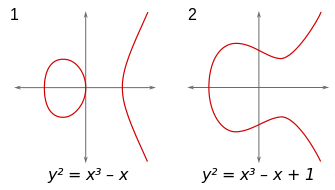
\includegraphics[width=200px]{ECC_1.png}
\end{figure}

Sulla sinistra una curva a due componenti, sulla destra una curva ad una componente.
Si hanno queste varianti in base alla cubica, si hanno infatti 3 radici che possono essere:
\begin{itemize}
    \item 3 reali $\implies$ curva a due componenti
    \item 1 reale e 2 complesse coniugate $\implies$ curva ad una componente
\end{itemize}

Si noti che sono sempre simmetriche rispetto all'asse delle $x$.
Se non imponessimo radici distinte avremmo curve con cuspidi o con nodi, in queste particolari curve la tangente non è detto che esiste unica.

La simmetria viene dal termine $y^2$, infatti:
$$ P = (x,y) \in E(a,b) \implies y^2 = x^3 + ax + b $$
definiamo dunque:
$$ -P = (x,-y) \implies (-y)^2 = y^2 = x^3 + ax + b $$

NB: si pone 0 = -0

Dato $P=(x,y) \in E(a,b) $ si dice \emph{opposto} e si indica con $-P$ il punto $-P=(x,-y)$.

\subsection{Somma sulla curva ellittica}
Non ha nulla a che fare con la somma delle coordinate!
Si parte da una curva e studiamo l'intersezione con una retta: si possono avere al massimo 3 punti di intersezione.
Si risolve infatti il sistema:
\begin{equation}
    \begin{cases}
    y = mx + q \\
    y^2 = x^3 + ax + b
    \end{cases}
\end{equation}
si ottiene una cubica che ha al massimo 3 soluzioni.

Il sistema può essere risolto con:
\begin{itemize}
    \item 1 solo punto reale e due complessi coniugati
    \item 3 reali
\end{itemize}

Posso quindi prendere due punti sulla curva P e Q dato che ho due intersezioni esplicite ce ne sarà una terza per forza, chiamiamolo $R$. Il risultato di questa somma sarà $-R$ (per definizione).

\begin{figure}[H]
    \centering
    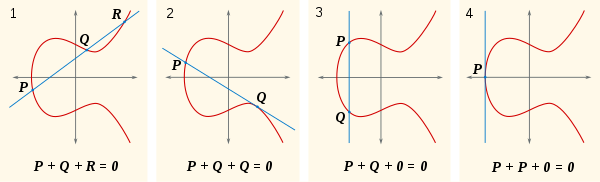
\includegraphics[width=325px]{ECC_2.png}
\end{figure}

Presi $P, Q, R \in E(a,b)$ se $P, Q, R$ sono disposti su una retta si pone:
$$ P + Q + R = 0 \implies P + Q = -R $$

Se $Q = P$ si considera la tangente alla curva nel punto $P$ (sempre definita per costruzione in quanto $4a^3+2tb^2 \neq 0$) e se ne vede l'intersezione con la curva.
Si noti che anche in questo caso se si fa passare una retta sull' estremo sinistro si ha una retta verticale e quindi la somma può dare il punto all'infinito.

\clearpage

\subsection{Proprietà della somma}
\subsubsection{Chiusura}
$$ \forall P, Q \in E(a,b): P+Q \in E(a,b) $$

\subsubsection{Elemento neutro}
$$ \forall P \in E(a,b): P + 0 = 0 + P = P $$

NB: Prendendo un punto $P$ e tracciando la retta all'infinito passante per $P$ l'altra intersezione è $-P$ quindi il risultato è $-(-P) = P$.

\subsubsection{Inverso (opposto)}
$$ \forall P \in E(a,b) \exists! Q \in E(a,b) : P + Q = 0 = Q + P$$
$$ Q = -P \implies P = (x,y), Q = (x, -y) $$

\subsubsection{Commutativa}
$$ \forall P, Q \in E(a,b) P + Q = Q + P $$

\subsubsection{Associativa}
$$ \forall P, Q, R \in E(a,b) (P + Q) + R = P + (Q + R) $$

\subsection{Formulazione algebrica}
Dati $P = (x_P, y_P)$, $Q = (x_Q, y_Q)$, $S = (x_S, y_S) = P+Q$ abbiamo:
\begin{itemize}
    \item $Q \neq \pm P$:
    \begin{equation}
        \begin{cases}
            x_S = \lambda^{2} - x_P - x_Q \\
            y_S = -y_P + \lambda(x_P + x_S) \\
            \lambda = \frac{y_Q - y_P}{x_Q - x_P}
        \end{cases}
    \end{equation}
    \item $P = Q$:
    \begin{equation}
        \begin{cases}
            x_S = \lambda^{2} - x_P - x_Q \\
            y_S = -y_P + \lambda(x_P + x_S) \\
            \lambda = \frac{3x_P^{2} + a}{2y_P}
        \end{cases}
    \end{equation}
    
    NB: se $y_P = 0$ $P+P=0$
    \item $Q = -P \implies P+Q = 0$
\end{itemize}

\subsection{Curve ellittiche su campi finiti}
\begin{minipage}{0.45\textwidth}
\centering
    Curve prime
    
    $K = Z_p$
    
    $p$ primo
    
    la caratteristica di $Z_p$ è $p$ quindi imponiamo $ p > 3 $
\end{minipage}
\hfill
\begin{minipage}{0.45\textwidth}
\centering
    Curve binarie
    
    $K = GF(2^m) , m \in \mathbb{N}$
    
    la caratteristica di K è uguale a 2 quindi non si può usare la forma normale di Weierstrass
\end{minipage}

Noi consideriamo solo le curve prime per le quali $4a^3 + 27b^2 \mod p \neq 0$ (CNS per gruppo Abeliano).

Ridefiniamo quindi la curva:
$$ E_p(a,b) = \{ (x,y) \in Z_p^2 \mid y^2 \mod p = x^3 + ax + b \mod p \} \cup \{0\} $$

Si noti che essendo in modulo si lavora sempre nel primo quadrante: $x, y \geq 0$.
La curva sarà ancora simmetrica ma non rispetto $y = 0$, bensì rispetto $y = \frac{p}{2}$ (parte intera inferior).

Inoltre tutti i valori saranno in $[0, p-1]$ per il modulo.

Essendo simmetrica se $P=(x,y) \in E_p(a,b) \implies -P = (x, p-y) \in E_p(a, b)$.

NB: se $y^2 \equiv x^3 + ax + b$ allora $(p-y)^2 \equiv p^2 -2py + y^2 \equiv y^2$

Le formule della somma sono dunque le stesse ma si lavora in modulo (le divisioni diventano moltiplicazioni per l'inverso se non ci sono semplificazioni immediate, l'inverso c'è sempre perché lavoriamo modulo un numero primo).

\subsection{Ordine di una curva}
L'ordine di una curva è il numero di punti che la curva possiede.
Si hanno al massimo $p$ valori per $x$ quindi mi aspetto circa $2p + 1$ valori di $y soluzioni$.
Ovviamente non tutti i valori nel campo hanno una radice quindi sono molti meno di $2p + 1$.
In genere in $Z_p$ i residui quadratici che definiscono un punto sulla curva sono $\frac{p-1}{2}$.

Il teorema di \emph{Hasse} ci dice che se $N$ è l'ordine della curva prima $E_p(a,b)$ allora:
$$ \mid N - (p+1) \mid \leq 2\sqrt{p}  $$

\subsection{Costruzione di una funzione one-way trap-door}
C'è una specie di parallelismo tra le operazioni in algebra modulare e le operazioni sulla curva ellittica:
\begin{itemize}
    \item la moltiplicazione diventa la somma tra due punti
    \item l'elevamento a potenza $k$ diventa la moltiplicazione di un punto per lo scalare $k$
\end{itemize}

Ci servono algoritmi di costo polinomiale quindi fare la somma $k$ volte non è praticabile (sarebbe esponenziale nella dimensione di $k$).
Possiamo quindi riusare l'algoritmo della esponenziazione veloce adattandolo: \emph{algoritmo dei raddoppi ripetuti}.

Eseguire $Q = kP$ si fa quindi in tempo polinomiale, trovare $k$ tale che $Q = kP$ invece è un problema difficile, si parla di \emph{logaritmo discreto sulle curve ellittiche}.

\subsection{Moltiplicazione scalare}
Calcolare $Q = kP$ è one-way, dati $k$ e $P$ è infatti facile calcolare $Q$ e si fa in O($\log k$):

Dato $Q = kP$, riscrivo $k$ in notazione binaria: 
$$ k = \sum_{i=0}^{t}k_i \cdot 2^i = (k_t,k_{t-1},\_,k_2,k_1,k_0) $$

Mi servono quindi $t+1 = \lfloor \log_2 k \rfloor + 1$ bit.
Si calcolano i vari $2P, 4P, \_, 2^tP$ in $t$ raddoppi ciascuno come raddoppio del punto precedente.
Si calcola $Q = \sum_{i : k_i = 1} (2^iP)$ in esattamente $t somme$.

O($t$) = O($\log_2 k)$ quindi lineare nella dimensione dell'input.

vediamo l'inverso della moltiplicazione scalare: dati $P$ e $Q$, sulla curva $E_p(a,b)$, trovare il più piccolo $k$ tale che: $Q = kP$. Non si conoscono algoritmi polinomiali ne sub-esponenziali per risolvere il problema.

\subsection{Protocollo DH su curve ellittiche}
Alice e Bob scelgono una curva ellittica prima (che soddisfi la condizione di gruppo Abeliano) ed un punto $B$ della curva che abbia ordine molto grande (l' ordine di un punto è il più piccolo $n$ tale che $nB=0$).

$B$ sarebbe il generatore di DH.

NB: i punti e le curve sono già consigliate da NIST, non si devono quindi creare da zero.
Sono note e pubbliche.

L'algoritmo prosegue così:
\begin{itemize}
    \item Alice estrae $n_A < n$ casuale, calcola $P_A = n_AB$ e lo invia in chiaro a Bob
    \item Bob riceve $P_A$. Estrae $n_B < n$ casuale, calcola $P_B = n_BA$ e lo invia in chiaro ad Alice
    \item Alice riceve $P_B$ e calcola $S = n_AP_B = n_An_BP$
    \item Bob riceve $P_A$ e calcola $S = n_BP_A = n_Bn_AP$
\end{itemize}
ambo le parti hanno generato lo stesso $S$ e possono quindi generare la stessa chiave di sessione in vari modi (ad esempio $K = x_S \mod 256$).

Un crittoanalista non può fare nulla perché conosce $E_p(a,b), B, n, P_A, P_B$ ma non può trovare $n_A$ o $n_B$ se non risolvendo il problema del logaritmo discreto su curva ellittica.

NB: è sempre possibile un man-in-the-middle quindi la chiave va sempre estratta da un certificato!

NB: il sistema col logaritmo discreto su curva ellittica è facile sulla macchina quantistica.

\subsection{Scambio di messaggi cifrati}

\subsubsection{Algoritmo di Koblitz}
Innanzitutto bisogna preparare il messaggio affinché sia utilizzabile.
Si mappa quindi $m$ ad un punto della curva ellittica:
$$ m \xrightarrow{} P_m \in E_p(a,b) $$
si potrebbe pensare di usare $m$ come $x$ del punto ma potremmo incappare in una $y^2$ che non è un residuo quadratico, succede ben in $\frac{1}{2}$ delle volte.
Si usa quindi \emph{l'algoritmo di Koblitz} che prende un intero $n$ e restituisce un punto sulla curva.
E' un algoritmo randomizzato.

Si sceglie $h$ intero tale che $(m + 1) \cdot h < p$, eseguo quindi $i$ tentativi calcolando $x = m \cdot h + i$ con $0 \leq i < h$ e vedo se ottengo un punto valido:

\begin{verbatim}
    KOBLITZ(m, h, E):
        for(i=0; i < h; i++):
            x = m*h + i
            z = (x^3 + E.a*x + E.b) mod E.p
            if z è un residuo quadratico:
                y = sqrt(z)
                return (x,y)
        return "failure"
\end{verbatim}

La probabilità di fallimento è $\approx \frac{1}{2}^h$, quindi la probabilità di successo è circa $\approx 1 - \frac{1}{2}^h$.

Se ci è andata male si modifica il messaggio e si riprova.

In fase di decriptazione si ritrovano $(x,y)$ ma $x$ non è il messaggio vero, si deve infatti calcolare:
$$ m = \lfloor \frac{x}{h} \rfloor = \lfloor \frac{mh+i}{h} \rfloor = \lfloor m + \frac{i}{h} \rfloor = m $$

\subsubsection{Cifratura e decifratura}
Presi una curva $E_p(a,b)$ ed un suo punto $B$ con ordine elevato $n$, preso inoltre $h$ da usare per Koblitz ogni utente deve generare la sua coppia chiave pubblica-chiave privata.

\begin{itemize}
    \item Bob U estrae $n_{BOB} < n$, chiave privata
    \item calcola $P_{BOB} = n_{BOB} \cdot B$, chiave pubblica
\end{itemize}

Ora Alice vuole inviare un messaggio cifrato a Bob:
\begin{itemize}
    \item prende il messaggio $m$ e lo mappa ad un punto della curva $P_m \in E_p(a,b)$
    \item sceglie un intero a caso $r$, calcola $V = r \cdot B$. $V$ è un punto che \emph{protegge} $r$
    \item calcola $W = P_m + r \cdot P_{BOB}$
    \item invia la coppia $<V,W>$
\end{itemize}

Bob deve quindi decifrare il messaggio:
\begin{itemize}
    \item riceve la coppia $<V,W>$
    \item calcola:
        $$ W -n_{BOB} \cdot V = P_m + r \cdot P_{BOB} - n_{BOB} \cdot r \cdot B = $$
        $$ = P_m + \cancel{r \cdot n_{BOB} \cdot B} - \cancel{r \cdot n_{BOB} \cdot B} = P_m$$
    \item ottiene il messaggio calcolando:
        $$ m = \lfloor \frac{x}{h} \rfloor $$
\end{itemize}

La sicurezza è legata al logaritmo discreto in quanto Eve può:
\begin{itemize}
    \item partendo da $V$ trovare $r$ e decifrare con:
    $$W - r\cdot P_{BOB} = P_m + \cancel{r \cdot P_{BOB}} - \cancel{r \cdot P_{BOB}} = P_m$$
    ma per trovare $r$ bisogna risolvere $V = r \cdot B$
    
    \item partendo da $P_{BOB}$ può trovare $n_{BOB}$ e decifrare esattamente come fa Bob, ma anche qui c'è da risolvere $P_{BOB} = n_{BOB} \cdot B$
\end{itemize}

Si noti che inoltre $r$ è one-time quindi se si dovessere passare a brutare converrebbe comunque andare a ricavare la chiave privata.

\subsection{Sicurezza}
Per attaccare RSA, DH, El Gamal (su algebra modulare) si hanno algoritmi di costo O($2^{\sqrt{b \log b}}$) con $b$ numero di bit del modulo.

Questi attacchi sono basati sull' \emph{index calculus} in quanto si ha una struttura di campo.
Per attaccare protocolli su curve ellittiche invece si ha un costo O($2^{\frac{b}{2}}$) con $b$ bit dell'ordine di $B$, non essendo un campo ma un gruppo Abeliano si pensa che le tecnice usate per l'algebra modulare non verranno mai trasposte anche qui.